
\chapter{PCTFPM and Shishkin Mesh Theory}

\label{Chapter3} % For referencing the chapter elsewhere, use \ref{Chapter1} 

\lhead{Chapter 3. \emph{PCTFPM and Shishkin Mesh}}

The theory of some other concepts/methods which were encountered during the course of this thesis is described here.

\section{Parallelogram Centred Tailored Finite Point Method (PCTFPM)}

\begin{figure}[htbp]
	\centering
		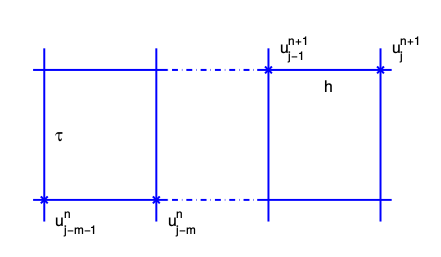
\includegraphics[height=4cm]{Figures/mesh_PCTFPM.png}\\
	\caption[RCTFPM imaginary part]{}
\end{figure}
The parallelogram scheme is given as follows:
\begin{align*}
 u_{j}^{n+1} = \alpha_{-1}u_{j-1}^{n+1}+\beta_{-1}u_{j-m-1}^{n}+\beta_{0}u_{j-m}^{n}
\end{align*}

As seen from the mesh and from the scheme, there is a diagonal like correspondance between the points of the next time step and the current
time step. This can be useful whenever there is a discontinuity in the initial condition or an interior layer is being formed because 
of a discontinuous source term or a discontinuous coefficient.

By using the basis
\begin{align*}
 V = {\{} v(x,t)|v(x,t) =  c_{1} + c_{2}e^{(ik_{j}(at-x))} + c_{3}e^{-(ik_{j}(at-x))}, \hspace{0.5cm} \forall c_{1}, c_{2}, c_{3} \in \mathbb{C} {\}}  
\end{align*}

Taking the coeffecients $(c_1, c_2, c_3)$ as (1,0,0), (0,1,0), (0,0,1) we get
\begin{align*}
 1 &= \alpha_{-1} + \beta_{-1} + \beta_{0} \\
 cos(k_{j}a \tau ) &= \alpha_{-1}\cos(k_{j}(a \tau + h)) + \beta_{-1}\cos(k_{j}(m+1)h) + \beta_{0}\cos(mh)\\
 sin(k_{j}a \tau ) &= \alpha_{-1}\sin(k_{j}(a \tau + h)) + \beta_{-1}\sin(k_{j}(m+1)h) + \beta_{0}\sin(mh)
\end{align*}

Thus we get

\begin{align*}
 \alpha_{-1} &= \frac{\sin(k_{j}(a \tau -(m+1)h)/2)}{\sin(k_{j}(a \tau -(m-1)h)/2)}\\
 \beta_{-1} &= 1\\
 \beta_{0} &= -\alpha_{-1}
\end{align*}

PCTFPM is unconditionally stable and has second order convergence in space.


\section{Shishkin Mesh}

An approach to solving parabolic problem on a Shishkin mesh is described here.

The problem is as follows:

\begin{align*}
 &u_{t} - \epsilon u_{xx} + b u_{x} = 0 \text{ for } (x,t) \in \Omega = (0,1)\\
 &u(x,0) = \phi(x)\\
 &u(0,t) = \alpha(t), \hspace{5mm} u(1,t) = \beta(t)
\end{align*}

\begin{figure}[htbp]
	\centering
		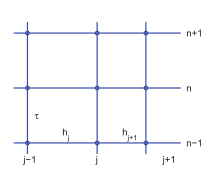
\includegraphics[height=4cm]{Figures/shiskin.png}\\
	\caption[RCTFPM imaginary part]{}
\end{figure}

\subsection{Construction of the mesh and an Implicit Scheme}
We consider the interval $[0,1]$. Let $\sigma = \max\{\frac{1}{2},1-\frac{2 \epsilon}{b}ln(N)\}$, where N is the number
of intervals in the mesh. The mesh is divided into $[0,\sigma]$ and $[\sigma,1]$ in $(N/2)$ equidistant parts.

\begin{align*}
x_{j} = \begin{cases} 
	    jH \hspace{1cm} \text{when} j \leq N/2\\
	    \sigma + (j-\frac{N}{2})h \hspace{1cm} \text{when} j>N/2\\
	 \end{cases}
\end{align*}

where
\begin{align*}
 H &= \frac{2 \sigma}{N}\\
 h &= \frac{2(1-\sigma)}{N}
\end{align*}

\begin{align*}
 u_{j}^{n} = a_{1}u_{j-1}^{n+1} + a_{2}u_{j}^{n+1} + a_{3}u_{j+1}^{n+1}
\end{align*}

The basis used is

\begin{align*}
 \{ 1, x-bt, e^{\frac{bx}{\epsilon}} \}
\end{align*}

Substituting these basis functions we get

\begin{align*}
 &a_{1}+a_{2}+a_{3} = 1\\
 &a_{1}(-h_{j})+a_{3}h_{j+1} = b \tau\\
 &a_{1}e^{-\frac{bh_{j}}{\epsilon}}+a_{2}+a_{3}e^{-\frac{bh_{j+1}}{\epsilon}} = 1
\end{align*}

Solving the above system leads to

\begin{align*}
 a_{1} &= \frac{b \tau (e^{bh_{j+1}/\epsilon}-1)}{h_{j+1}(1-e^{-bh_{j}/\epsilon}) - h_{j}(e^{bh_{j+1}/\epsilon}-1)}\\
 a_{3} &= \frac{b \tau (1-e^{-bh_{j}/\epsilon})}{h_{j+1}(1-e^{-bh_{j}/\epsilon}) - h_{j}(e^{bh_{j+1}/\epsilon}-1)}\\
 a_{2} &= 1-a_1-a_3
\end{align*}

Thus the above scheme can be used to solve parabolic problems on a Shishkin mesh.
